\chapter{Partial Redundancy Elimination}\label{ch:pre}

Given two expression X and Y in the source code, following are the possibilities -
\begin{enumerate}
% There is scope for condensing this. Maybe we can inline this and not write in point format
\item X and Y are lexically equivalent, and have the same value numbers
\item X and Y are lexically equivalent, but have different value numbers
\item X and Y are lexically different, but have the same value numbers
\item X and Y are lexically different, and have different value numbers
\end{enumerate}
In the source code, there could be opportunities for redundancy elimination in
cases 1, 2 and 3 above. If the source code is converted to an intermediate
representation in SSA form then case 2 becomes an impossibility (by guarantees of SSA). Therefore,
               our algorithm presently handles the cases when X and Y are
               lexically same/different, but both have the same value number (cases 1 and 3).
               Driven by this observation, we implement value number based code
               motion, the details of which are presented below. It should be
               noted that even though case 2 above is not possible in SSA,
               the source code redundancies  of this type transform into that
               of the form of case 4. Figure\ref{fig:1} is an example. One of our
               future work for the semester is to handle this case. % the last line should be in bold

\begin{figure}[htbp]
  \begin{center}
    \scalebox{.7}{\begin{tabular}{@{}p{12cm}@{ } @{ }p{12cm}@{}}
     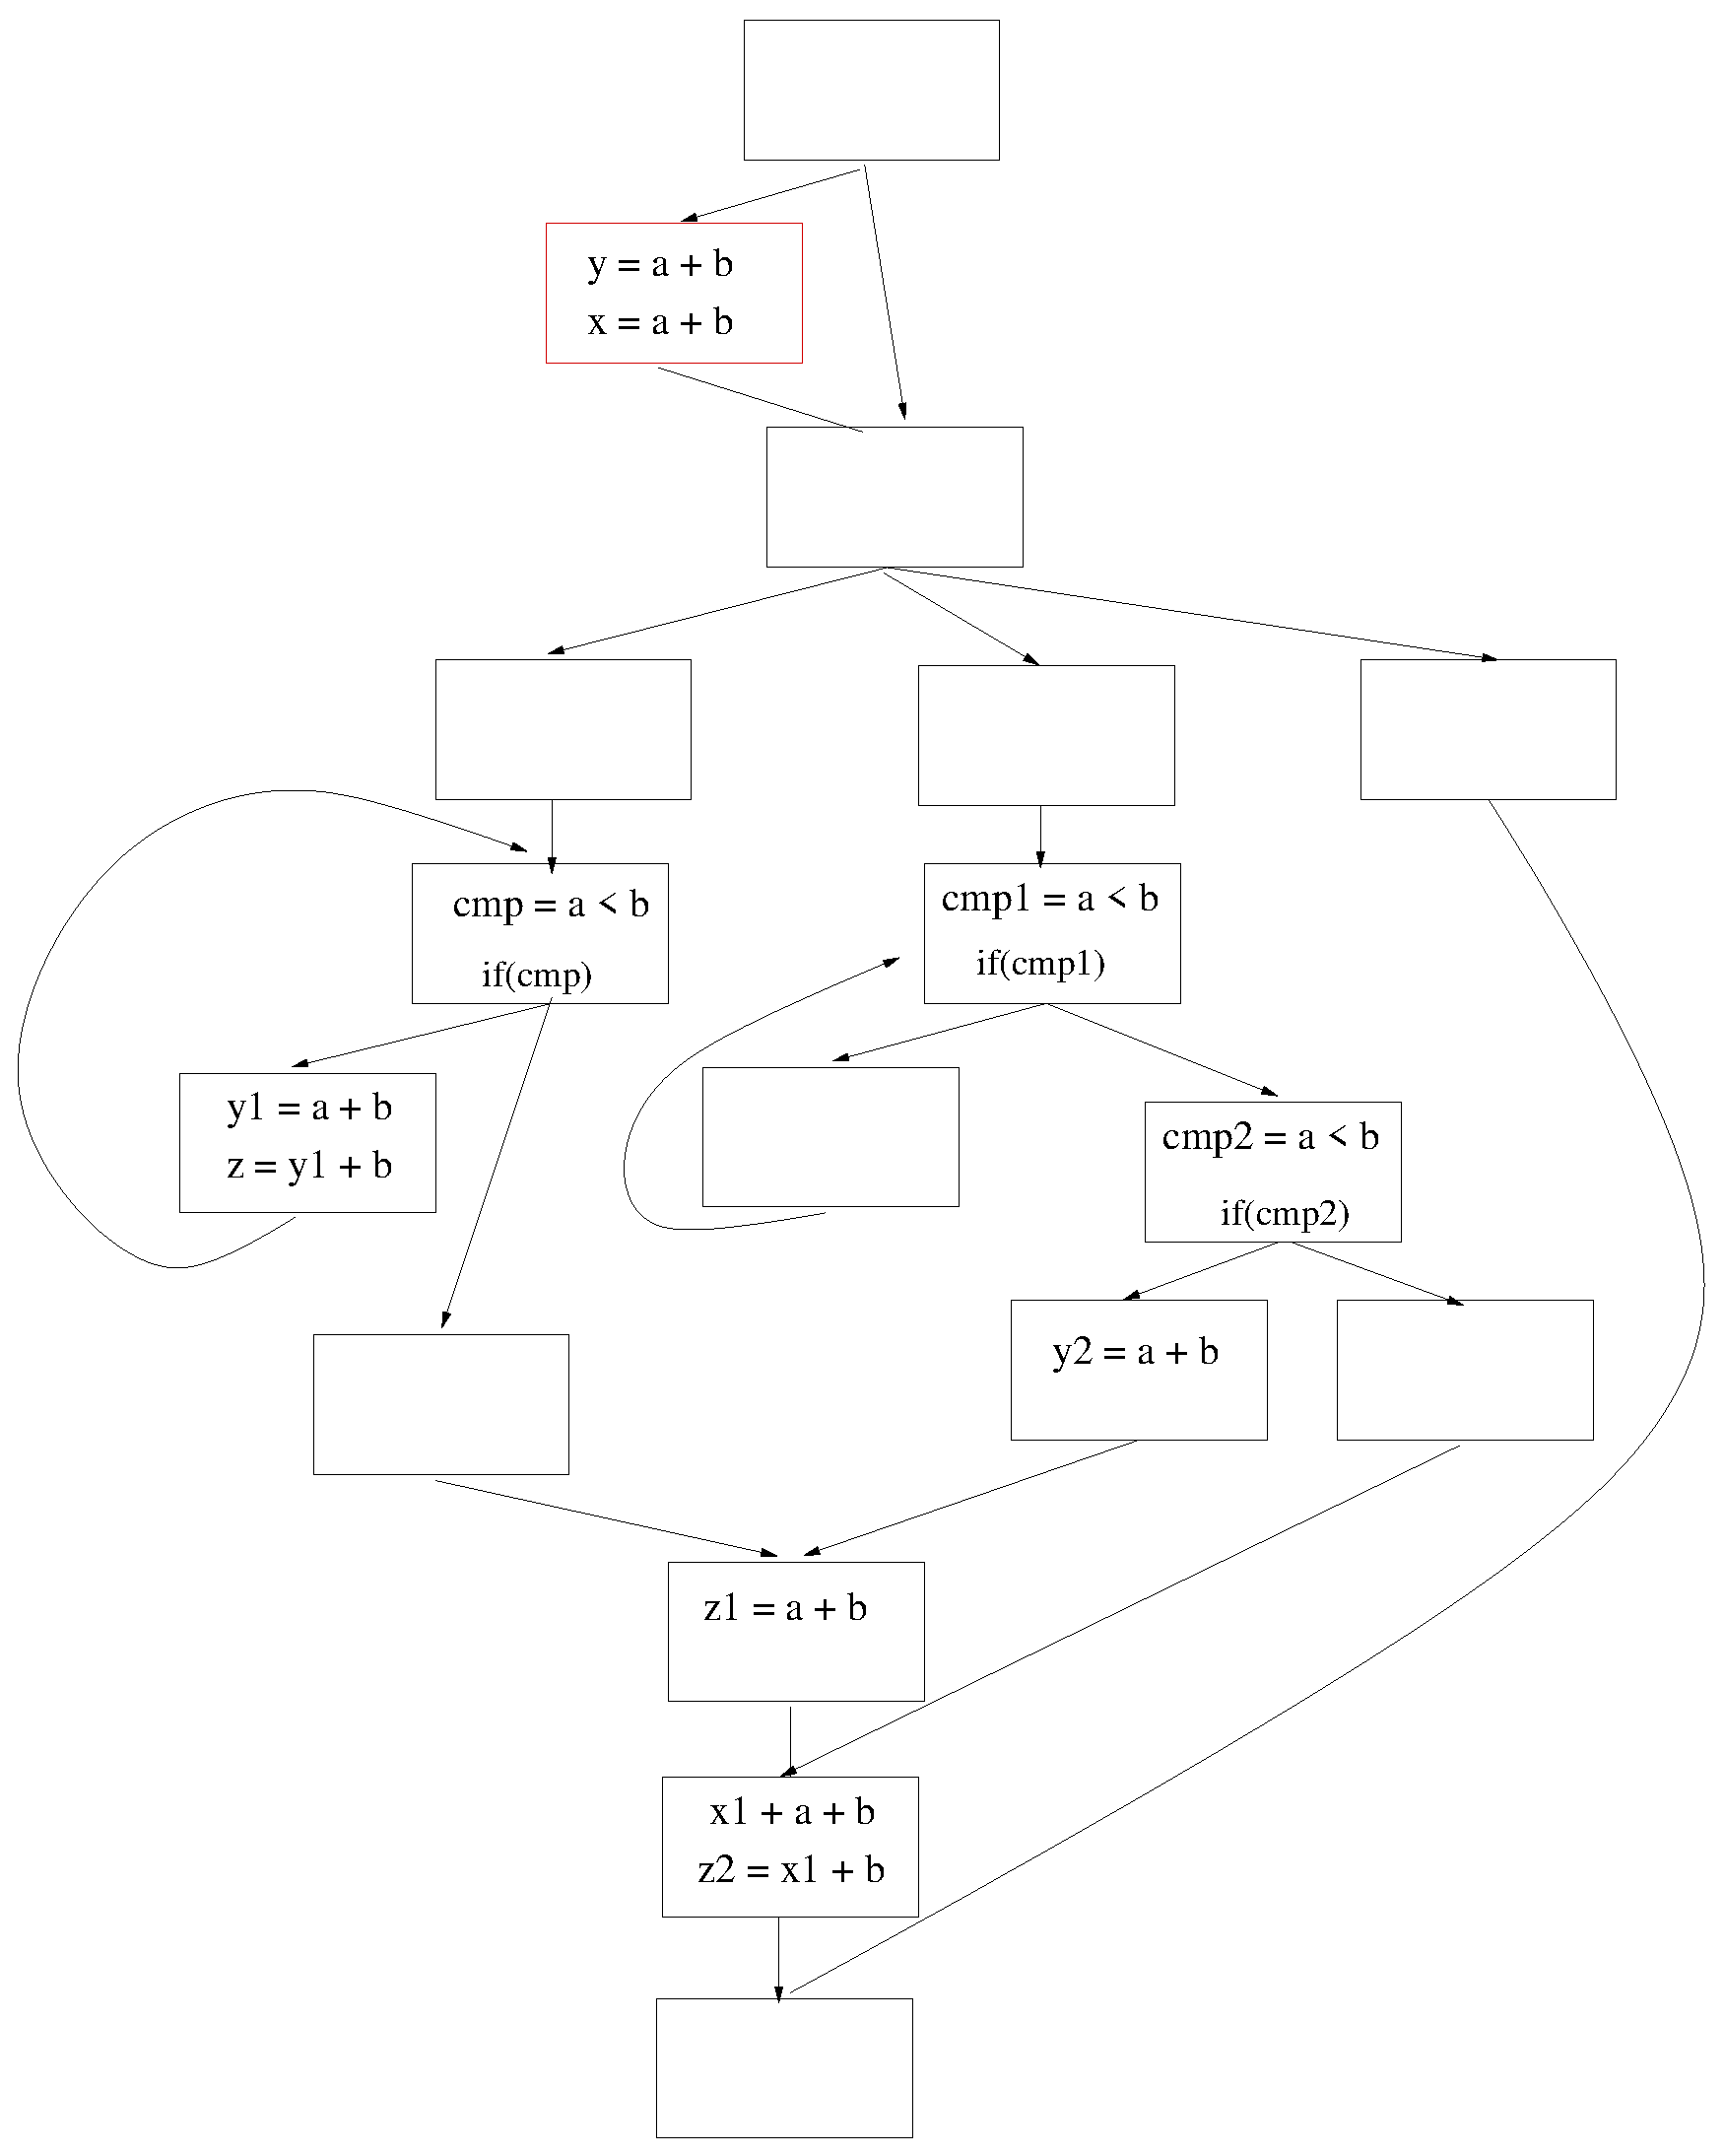
\includegraphics[scale=0.8]{1} & 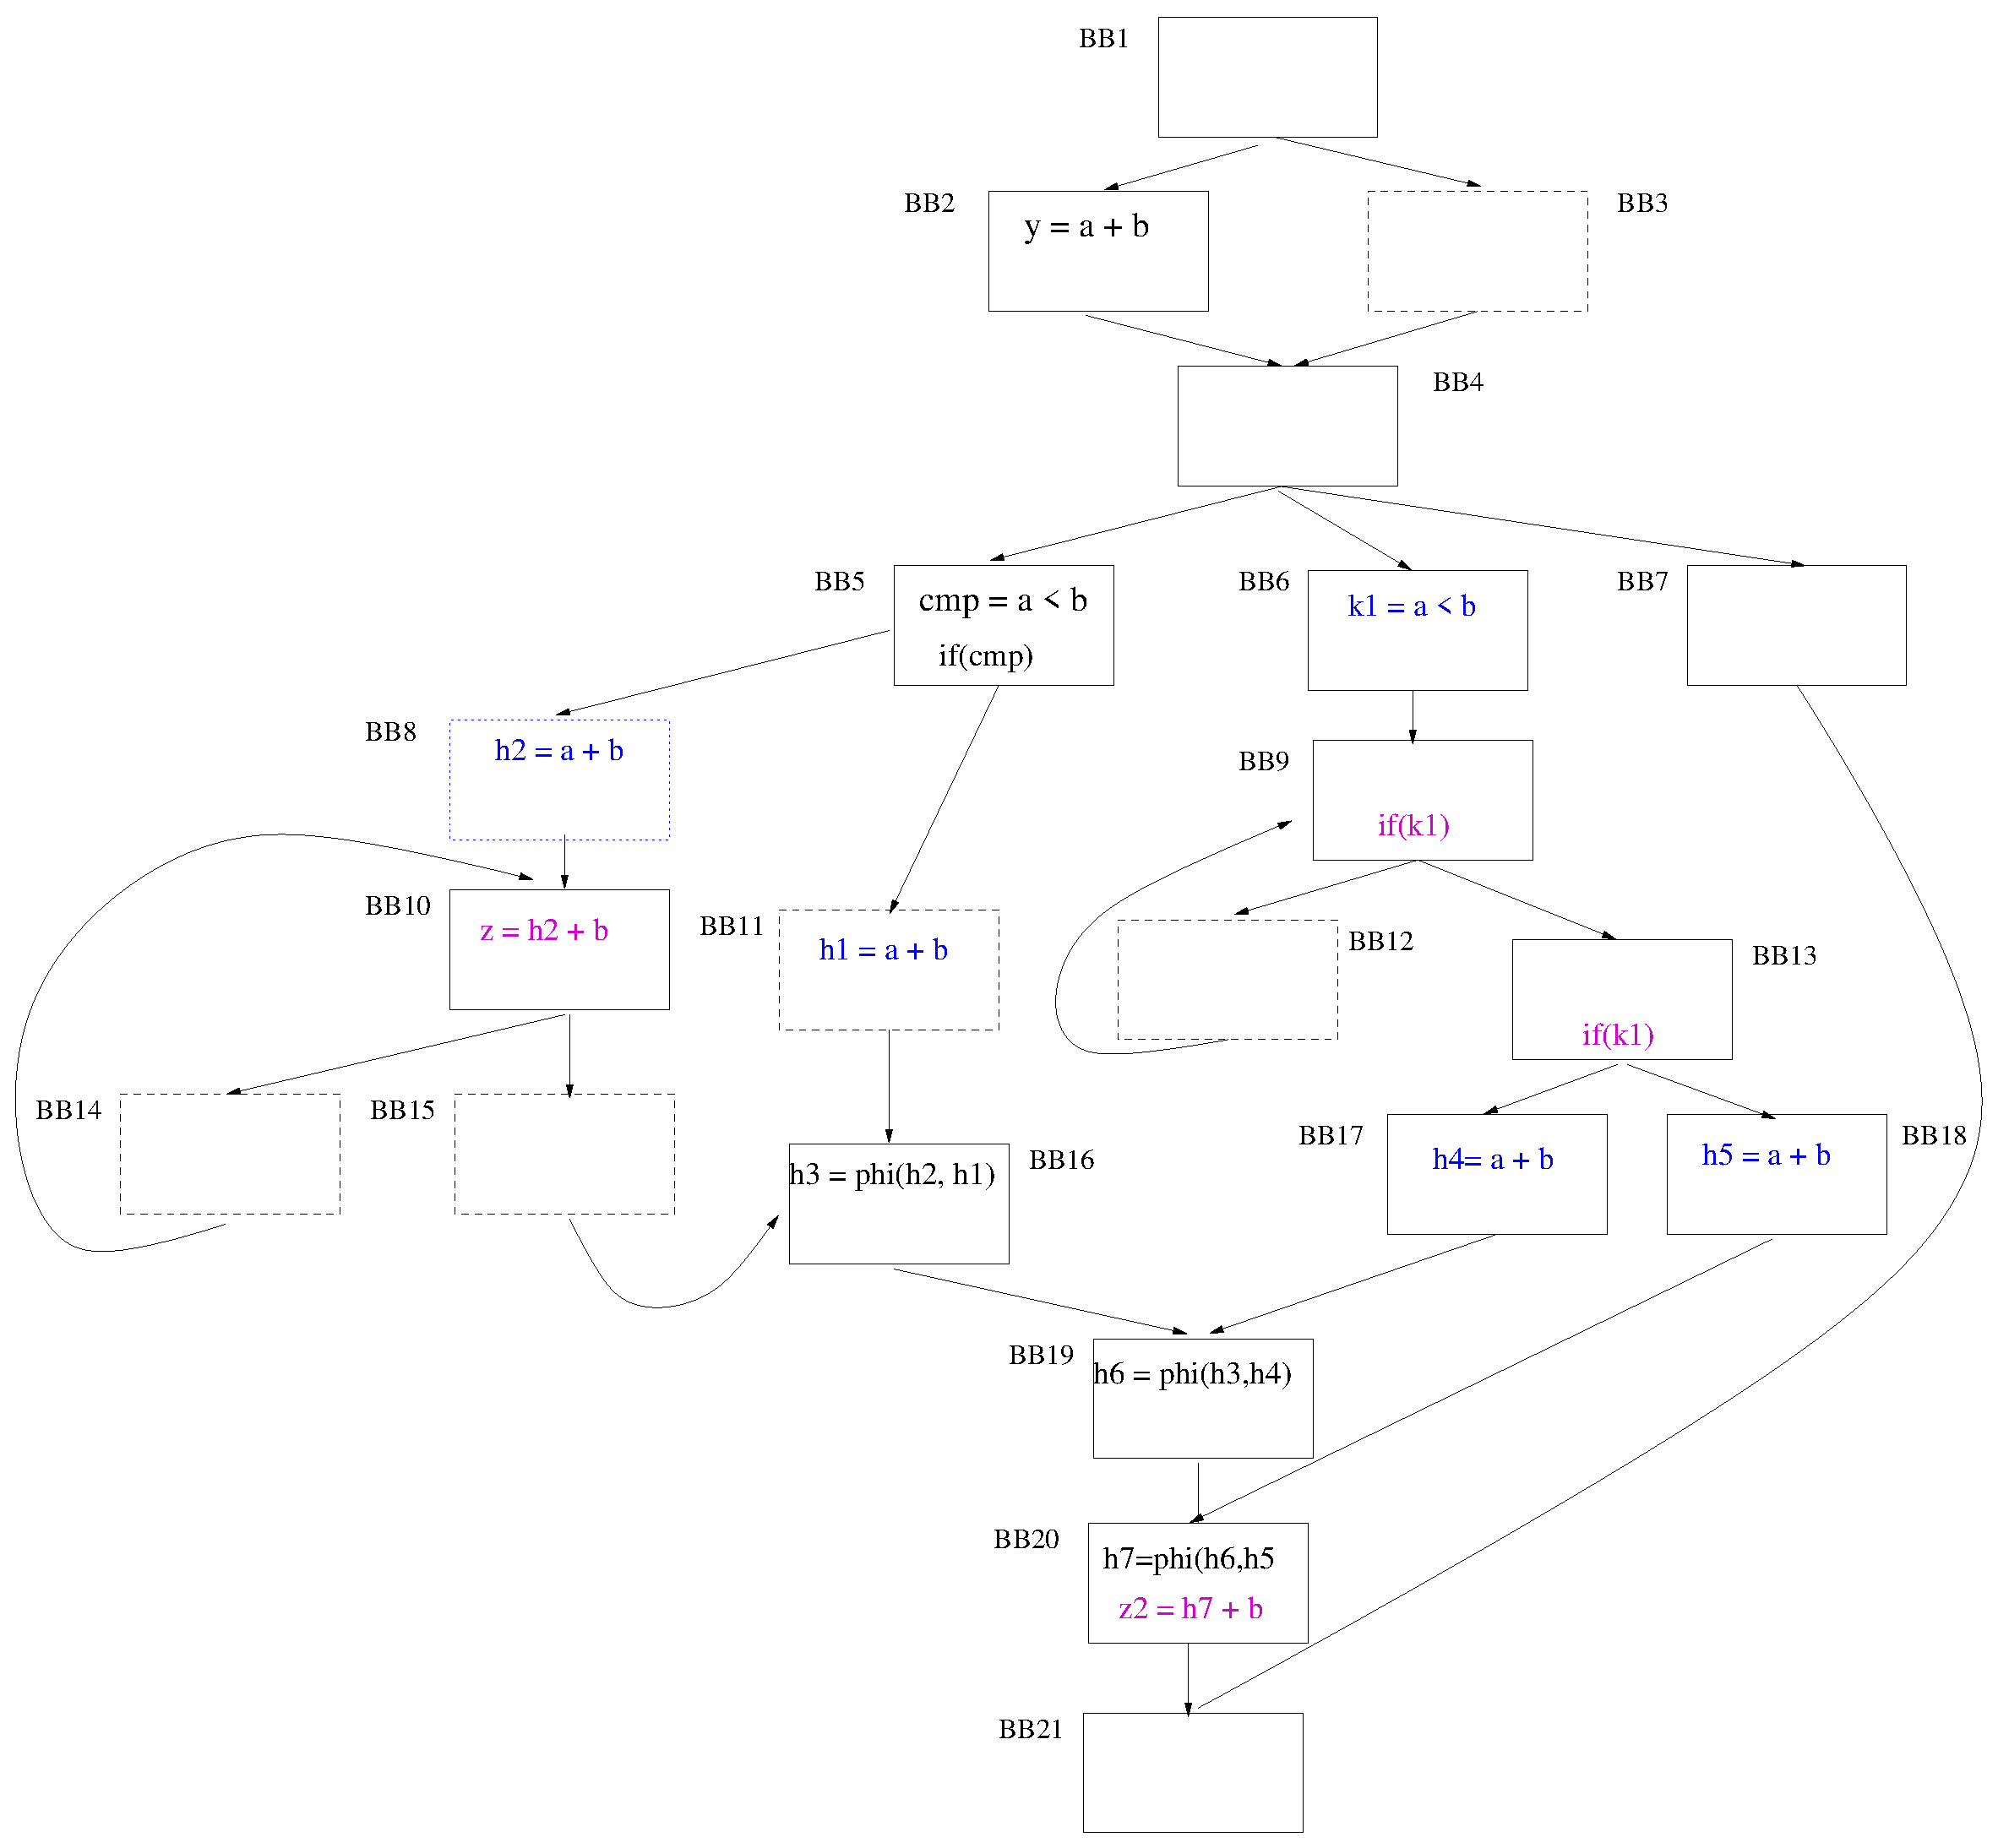
\includegraphics[scale=0.8]{2} \\
      &\\
  \text{Code not in SSA Form; Two lexically equivalent expressions} &
  \text{Code in SSA Form; Two lexically different expressions} \\
  \text{in Basic block 3 and 4 with different value numbers.} &
  \text{in Basic block 3 and 4 with different value numbers.}
    \end{tabular}}
  \end{center}
  \caption{\label{fig:1} }
\end{figure}
  
